\documentclass{beamer}

\usetheme{uhh}
\showtotalframenumber
\showuhhlogoeachframe
\showsections

\usepackage{amsmath}
\usepackage{graphicx}
\DeclareMathOperator*{\argmin}{arg\,min}

\usepackage{listings}
\lstset{
  language=python
  }

\title{Part 05: Neural Tagger with RNNs in Tensorflow}
\author{Fabian Barteld, Benjamin Milde}
\date[5.12.2018]{December 5, 2018}

\AtBeginSection[]
{
   %%%%% section title
   % This is how it would look like in Beamer:
   % \begin{frame}
   %     \frametitle{Overview}
   %     \tableofcontents[sections={2-3},currentsection,sectionstyle=show/hide,subsectionstyle=hide]
   % \end{frame}
  \begin{frame}[plain]
  \begin{tikzpicture}[overlay]
    \relax%
    \fill[blueuhh,opacity=1] (-10,-10)
    rectangle(\the\paperwidth,\the\paperheight);
  \end{tikzpicture}
   \begin{tikzpicture}[overlay]
    \relax%
    \fill[white,opacity=1] (-5,-1.2)
    rectangle(\the\paperwidth,0.5) node[pos=0.5,black]{\LARGE\insertsectionhead};
  \end{tikzpicture}
  \end{frame}

  %%%% add subsection to show navigation dots
  \subsection{}
}

\begin{document}

\maketitle

%\begin{frame}
%  \frametitle{Overview}
%
%  \tableofcontents
%
%\end{frame}

\section{Introduction}

\begin{frame}[fragile]
\frametitle{RNNs - different variants}
  \begin{itemize}
  	\item DNNs have an obvious limitation for NLP, they always need a fixed-sized input. Recurrent Neural Networks (RNNs) on the other hand operate on sequences of varying length \rightarrow ideal for text and speech
    \item Depending on the task, RNNs can be used in different ways
  	\item All of these are fairly straightforward to do in Tensorflow
  \end{itemize}
    \begin{center}
		\includegraphics[width=0.8\textwidth]{05_rnn_variants}
	 \end{center}
\end{frame}

\begin{frame}[fragile]
\frametitle{RNNs}
  \begin{itemize}
  	\item Update a state given inputs at each timestep
  	\item Can be "unrolled" into a DNN:
  \end{itemize}
    \begin{center}
  		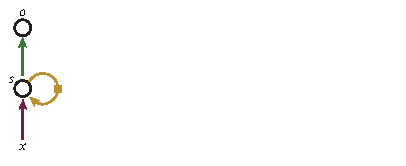
\includegraphics[width=0.7\textwidth]{05_RNN_schema}
  	\end{center}

\end{frame}

\begin{frame}[fragile]
\frametitle{RNNs}
  \begin{itemize}
  	\item Update a state given inputs at each timestep
  	\item Can be "unrolled" into a DNN:
  \end{itemize}
  \begin{center}
  	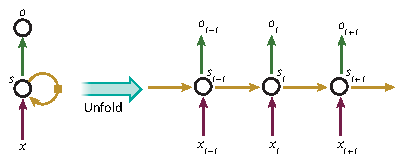
\includegraphics[width=0.7\textwidth]{05_RNN_schema_unfold}
  \end{center}
\end{frame}

\begin{frame}[fragile]
\frametitle{LSTMs - intuition}
  \begin{itemize}
  	\item Vanilla RNNs are difficult to train: the same operation is applied at ever time step - difficult to optimize for many time steps (vanishing and exploding gradients)
	\item When we use RNNs, we usually use a variant that has a gating mechanism
	\item Intuition: sometimes we need to forget things, also we want to learn how much to change our internal state given certain inputs
	\item Hochreiter, S. and Schmidhuber, J. (1997). Long short-term memory. Neural computation, 9(8), 1735-1780.
  \end{itemize}
\end{frame}

%\begin{frame}[fragile]
%\frametitle{LSTMs}
%  \begin{itemize}
%\item Input gate - network decides whether each cell (individually) is going to observe input (or ignore it)
%\item Forget gate - network decides for each cell whether it should be kept or forgotten (set to 0)
%\item Output gate - network decides whether a cell should be shown to other cells and to the next layer.
%\begin{center}
%	\includegraphics[width=0.5\textwidth]{05_lstm}
%\end{center}
%  \end{itemize}
%\end{frame}

\begin{frame}[fragile]
\frametitle{Understanding LSTMs}
  \begin{itemize}
	\item All graphics and some of the explanations on this and on the following slides are from: \url{http://colah.github.io/posts/2015-08-Understanding-LSTMs/}
	\item  The repeating module in a standard RNN contains a single layer:	
\begin{center}
	\includegraphics[width=0.6\textwidth]{05_LSTM3-SimpleRNN}
\end{center}
  \end{itemize}
\end{frame}

\begin{frame}[fragile]
\frametitle{Understanding LSTMs}
  \begin{itemize}
	\item An LSTM cell has more complex operations:
	\begin{center}
	\includegraphics[width=0.8\textwidth]{05_LSTM3-chain}
\end{center}
\begin{center}
	\includegraphics[width=0.8\textwidth]{05_LSTM2-notation}
\end{center}
  \end{itemize}
\end{frame}

\begin{frame}[fragile]
\frametitle{Understanding LSTMs}
  \begin{itemize}
	\item The key to LSTMs is the cell state.
	\item It runs straight down the entire chain, with only some minor linear interactions.
	\item It makes it easy for information to just flow along unchanged.
\begin{center}
	\includegraphics[width=0.8\textwidth]{05_LSTM3-C-line}
\end{center}
  \end{itemize}
\end{frame}

\begin{frame}[fragile]
\frametitle{Understanding LSTMs}
  \begin{itemize}
	\item Another key element of an LSTM cell is gating. A gate consists of a sigmoid layer and a multiplication.
	\item The sigmoid pushes all values to be between 0 and 1
	\item You can think of it as some kind of "differentiable Transistor"
\begin{center}
	\includegraphics[width=0.2\textwidth]{05_LSTM3-gate}
\end{center}
  \end{itemize}
\end{frame}


\begin{frame}[fragile]
\frametitle{Understanding LSTMs}
  \begin{itemize}
	\item The first step in an LSTM is to decide what information is going to be thrown away from the cell state.
	\item This decision is made by the "forget gate layer"
	\item It concatenates $h_{t−1}$ and $x$, applies a sigmoid layer and multiplies the output with the cell state.
 \vspace{-6mm}
\begin{center}
	\includegraphics[width=1.0\textwidth]{05_LSTM3-focus-f}
\end{center}
  \end{itemize}
\end{frame}

\begin{frame}[fragile]
\frametitle{Understanding LSTMs}
  \begin{itemize}
	\item The next step is to decide what new information we're going to store in the cell state. 
	\item First, a sigmoid layer called the "input gate layer" decides which values we'll update. Next, a tanh layer creates a vector of new candidate values, $C\~t$. 
	\vspace{-6mm}
\begin{center}
	\includegraphics[width=1.0\textwidth]{05_LSTM3-focus-i}
\end{center}
  \end{itemize}
\end{frame}

\begin{frame}[fragile]
\frametitle{Understanding LSTMs}
  \begin{itemize}
	\item Now the new cell state is calculated 
	\item We multiply the old state by $f_t$, forgetting the things we decided to forget earlier. 
    \item Then we add $i_t \cdot C\~t$. This is the new candidate values, scaled by how much we decided to update each state value.
    \vspace{-6mm}
\begin{center}
	\includegraphics[width=1.0\textwidth]{05_LSTM3-focus-C}
\end{center}
  \end{itemize}
\end{frame}

\begin{frame}[fragile]
\frametitle{Understanding LSTMs}
  \begin{itemize}
	\item Finally we compute the output based on the cell state
	\item The first step is a sigmoid layer which decides what parts of the cell state we're going to output. 
	\item Then, we put the cell state through tanh (values between -1 and 1) and multiply it by the output of the sigmoid gate, so that we only output the parts we decided to.
	\vspace{-6mm}
\begin{center}
	\includegraphics[width=1.0\textwidth]{05_LSTM3-focus-o}
\end{center}
  \end{itemize}
\end{frame}

\begin{frame}[fragile]
\frametitle{Popular variant of LSTMs: GRU}
  \begin{itemize}
  	\item Combines the forget and input gates into a single "update gate."
  	\item It also merges the cell state and hidden state, and makes some other changes. 
  \end{itemize}
\begin{center}
	\includegraphics[width=1.0\textwidth]{05_LSTM3-var-GRU}
\end{center}
\end{frame}

\begin{frame}[fragile]
 \frametitle{LSTMs in Tensorflow}
  \begin{itemize}
		\item Good news! RNNs are first class citizens in Tensorflow, you don't have to code the gating mechanism on your own
		\item Two types of RNNs: static\_rnn and dynamic\_rnn, also many types of cells, e.g. LSTMs and GRUs.
		\item The so called static\_rnn expects a list of tensors, one for each step. Number must be known at graph creation time!
		\item Sequences of smaller length must be padded!
	\end{itemize}
			
\begin{footnotesize}
\begin{lstlisting}
 cell = tf.contrib.rnn.LSTMCell(num_hidden)
 list_of_tensors = [x_embedd[:,num] for num in range(seq_len)]
 outputs, state = tf.nn.static_rnn(cell, list_of_tensors,
  dtype=tf.float32)
\end{lstlisting}   
\end{footnotesize}   
	
\end{frame}

\begin{frame}[fragile]
 \frametitle{LSTMs in Tensorflow}
\begin{footnotesize}
\begin{lstlisting}
 outputs, state = tf.nn.static_rnn(cell, list_of_tensors,
  dtype=tf.float32)
\end{lstlisting}   
\end{footnotesize}   

 \begin{itemize}
  	\item outputs is a list of tensors (?, hidden\_size), one of these for each output.
  	\item For LSTMs, state is a tuple of c and h:
 \end{itemize}
			
\begin{center}
	\includegraphics[width=0.5\textwidth]{05_lstmtuple}
\end{center}
\end{frame}			

\begin{frame}[fragile]
\frametitle{Exercise 1 - Tagger with static\_rnn}
  \begin{itemize}
  \item Make sure you have the newest Tensorflow version! (python3 -m pip install - -upgrade tensorflow)
  	\item Extend the neural tagger from the previous exercises so that static\_rnn is used, instead of a DNN
  	\item As before, use a fixed length context window (e.g. left\_context=4, right\_context=0)
  	\item We provide you with a new exercise file (05\_dnn\_tagger\_lstm\_ex.py): the solution for the tagger from previous exercises, which you need to extend.
  \end{itemize}
\end{frame}

\begin{frame}[fragile]
\frametitle{Variable sequence lengths}
  \begin{itemize}
  	\item Using a fixed length RNN isn't all to practical for NLP
  	\item Ideally, we would like to keep the sequence length dynamic
  	\item E.g. change it from batch to batch, as needed
  	\item Ideally we would like to operate on an input tensor shape like (None, None) - we don't know the batch size nor the sentence lengths in advance!
  	\item That's what dynamic\_rnn is for!	
  \end{itemize}
  
  \begin{footnotesize}
\begin{lstlisting}
cell = tf.contrib.rnn.LSTMCell(num_hidden)
output, state = tf.nn.dynamic_rnn(cell, x_embedd,
  dtype=tf.float32, sequence_length=seq_len_in)
\end{lstlisting}   
\end{footnotesize}   

\end{frame}

\begin{frame}[fragile]
 \frametitle{Variable sequence lengths}
\begin{footnotesize}
\begin{lstlisting}
output, state = tf.nn.dynamic_rnn(cell, x_embedd,
  dtype=tf.float32, sequence_length=seq_len_in)
\end{lstlisting}   
\end{footnotesize}   

 \begin{itemize}
  	\item output is a tensor, e.g. (?, ?, hidden\_size)
  	
  	\item For LSTMs, state is again a tuple of c and h. This is dependent on what you use as cell! E.g. with GRUs, there is no separate cell state $c$ in the cell.
 \end{itemize}
			
\end{frame}		

\begin{frame}[fragile]
\frametitle{Exercise 2 - Tagger with dynamic\_rnn}
  \begin{itemize}
  	\item Extend the neural tagger from the previous exercises so that dynamic\_rnn is used, instead of a DNN
  	\item There is a new prepare\_data\_sentences function for preparing the data, which you must use. Instead of a window, one training example is now a complete sentence.
  	\item Hints: you need to adapt inputs, also reshape the outputs of the rnn so that the loss function can be applied correctly.
	
  \end{itemize}
\end{frame}

\begin{frame}[fragile]
\frametitle{Exercise 2 - Things to try}
  \begin{itemize}
  	\item Bidirectional RNNs (e.g. tf.nn.bidirectional\_dynamic\_rnn)
  	\item Stacking RNNs (tf.contrib.rnn.MultiRNNCell, tf.contrib.rnn.stack\_bidirectional\_dynamic\_rnn)
  	\item Dropout for RNNs (tf.contrib.rnn.DropoutWrapper)
  \end{itemize}
\end{frame}

%\begin{frame}[fragile]
%  \frametitle{Layer based APIs vs. Graphs based}
%  
%Disadvantage: Difficult to express structures like these:
%  
%    \includegraphics[angle=-90,width=0.75\textwidth]{graph_example}
%
%Increasing evidence that these kind of deeply connected networks are very useful.
%  
%\end{frame} 
%
%\begin{frame}[fragile]
%  \frametitle{Layer based APIs vs. Graphs based}
%  \begin{itemize}
%		\item  Since Tensorflow uses computation graphs, the declaration of the model allows for a higher expressivity
%		\item  Has a steeper learning curve in the beginning
%		\item  In the newer versions of tensorflow, you can also mix layer-like APIs with the computation graph
%		\item  We will focus on not using any short cuts, as this has a higher learning effect and only make use of standard ops in the beginning
%  \end{itemize}
%\end{frame} 
%
%\begin{frame}[fragile]
%\frametitle{First steps - Lets open spyder}
%
%\includegraphics[width=1.0\textwidth]{spyder}
%
%\end{frame} 
%
%\begin{frame}[fragile]
%\frametitle{First steps - Necessary imports}
%
%\begin{lstlisting}
%import numpy as np
%import tensorflow as tf
%\end{lstlisting}
%
%\begin{itemize}
% 	\item Outside of graph computations, we usually store data in Numpy arrays.
% 	\item Numpy arrays are the main objects to transfer data to inputs of the graph and from outputs of the graph.
% 	\item Numpy arrays are also an abstraction for (homogeneous) multidimensional arrays.
%\end{itemize}
%
%\end{frame} 
%
%\begin{frame}[fragile]
%\frametitle{Generating some random data}
%
%\begin{lstlisting}
%#some random test data
%a_data = np.random.rand(256)
%b_data = np.random.rand(256)
%\end{lstlisting}
%
%\begin{itemize}
%	\item Now a and b contain vectors of length 256 with random floats. E.g. print(a\_data) returns:
%\end{itemize}
%
%\begin{lstlisting}
%[ 0.54976368  0.87790201  0.96528541 ..., 
% 0.05281365  0.48556404  0.46848266]
%  \end{lstlisting}
%
%\end{frame} 
%
%
%\begin{frame}[fragile]
%\frametitle{Declare the computation graph}
%
%\begin{lstlisting}
%#construct the graph
%a = tf.placeholder(tf.float32, [256])
%b = tf.placeholder(tf.float32, [256])
%
%x = a+b 
%\end{lstlisting}
%
%\begin{itemize}
%\item The placeholders can later be used to input data to the computation graph
%\item The operation x = a+b does not immediatly add something, it creates a graph.
%\item In fact, print(x) returns: 
%\end{itemize}
%
%\begin{lstlisting}
%Tensor("add:0", shape=(256,), dtype=float32)
%\end{lstlisting}
%
%\end{frame} 
%
%\begin{frame}[fragile]
%\frametitle{A session on a computation device}
%
%\begin{lstlisting}
%with tf.device('/cpu'):
%    with tf.Session() as sess:
%       x_data = sess.run(x, {a: a_data, b: b_data})  
%       print(x_data)
%\end{lstlisting}
%
%\begin{itemize}
%\item This fills the inputs a and b with a\_data and b\_data (our random data), runs the computation graph and retrieves the results of x in x\_data
%\item Obviously not terrible useful as is, but you could run the operation easily on a gpu by changing tf.device('/cpu') to  tf.device('/gpu:1'). Copying data to and from the GPU is handled automatically for you.
%\end{itemize}
%
%\end{frame} 
%
%\begin{frame}[fragile]
%\frametitle{Small warm up exercise!}
%
%\begin{itemize}
%	\item We change a and b to random matrices:
%\end{itemize}
%
%\begin{lstlisting}
%a = np.random.rand(256, 128)
%b = np.random.rand(128, 512)
%\end{lstlisting}
%
%\begin{itemize}
%	\item Calculate the resulting matrix of shape (256, 512) in TensorFlow.
%\end{itemize}
%
%\end{frame} 

%\section{Simple Optimization}
%
%% https://medium.com/@saxenarohan97/intro-to-tensorflow-solving-a-simple-regression-problem-e87b42fd4845
%% https://github.com/aymericdamien/TensorFlow-Examples/blob/master/examples/2_BasicModels/linear_regression.py
%\begin{frame}
%  \frametitle{Linear Regression}
%
%  \begin{itemize}
%  \item Given: $(x_1, y_1)$, \ldots, $(x_n,y_n)$
%  \item Goal: find $w$ and $b$ such that:
%    \begin{displaymath}
%      \argmin_{w, b} \frac{\sum^n_{i=1} (\hat{y}_i - y_i)^2}{n}
%    \end{displaymath}
%    where $\hat{y}_i = wx_i + b$.
%  \end{itemize}
%
%\end{frame}
%
%\begin{frame}[fragile]
%  \frametitle{Define model parameters}
%  Model: $\hat{y}_i = wx_i + b$
%
%\begin{lstlisting}
%w = tf.Variable(np.random.randn(), name="weight")
%b = tf.Variable(np.random.randn(), name="bias")
%\end{lstlisting}
%\end{frame}
%
%\begin{frame}[fragile]
%  \frametitle{Define the model}
%
%  \begin{displaymath}
%    \begin{pmatrix} \hat{y}_1\\\vdots\\\hat{y}_n\end{pmatrix} =
%    \begin{pmatrix} w\\\vdots\\w\end{pmatrix} *
%    \begin{pmatrix} \hat{x}_1\\\vdots\\\hat{x}_n\end{pmatrix} +
%    \begin{pmatrix} b\\\vdots\\b\end{pmatrix}
%  \end{displaymath}
%
%\begin{lstlisting}
%yhat = tf.add(tf.multiply(X, w), b)
%\end{lstlisting}
%
%{\footnotesize The scalars $w$ and $b$ are converted into vectors of the same
%  length as X (broadcast); \url{https://www.tensorflow.org/performance/xla/broadcasting}}
%
%\end{frame}
%
%\begin{frame}[fragile]
%  \frametitle{Define the loss}
%
%\begin{lstlisting}
%loss = tf.reduce_mean(tf.square(y - yhat))
%\end{lstlisting}
%
%\end{frame}
%
%
%\begin{frame}[fragile]
%  \frametitle{Optimization}
%
%\begin{lstlisting}
%epochs = 10
%optimizer = tf.train.GradientDescentOptimizer(
%    learning_rate).minimize(loss)
%
%with tf.Session() as sess:
%    ## initalize parameters
%    sess.run(tf.global_variables_initializer())
%
%    for i in list(range(epochs)):
%        ## run one epoch
%        sess.run(optimizer)
%        ## print result and loss
%        print(sess.run(yhat) + ' ' + sess.run(loss))
%\end{lstlisting}
%
%\end{frame}
%
%\begin{frame}[fragile]
%  \frametitle{Hands on: Simple optimization}
%
%  \begin{enumerate}
%  \item Do a linear regression to learn $y = 2x + 1$
%  \item Do a multiple linear regression with Boston housing prices
%  \end{enumerate}
%
%\begin{lstlisting}
%from sklearn.datasets import load_boston
%from sklearn.preprocessing import scale
%
%total_X, total_Y = load_boston(True)
%total_x = scale(total_x)
%\end{lstlisting}
%\end{frame}
%
%% https://www.tensorflow.org/tutorials/wide
%% https://github.com/aymericdamien/TensorFlow-Examples/blob/master/examples/2_BasicModels/logistic_regression.py
%\begin{frame}
%  \frametitle{Logistic regression}
%
%  TODO
%  tf.sigmoid
%
%\end{frame}
%
%\begin{frame}
%  \frametitle{Hands on: Regression model}
%
%  TODO: more complex example
%\end{frame}

\end{document}


%%% Local Variables:
%%% mode: latex
%%% TeX-engine: luatex
%%% End:
